%==========================================================
% PART 4: a simulated Algerian network (Phase 4).
%==========================================================
% generated by scripts/export_explainer_phase4.py -- do not edit
\newcommand{\PfourRadarSigma}{0.59}
\newcommand{\PfourRadarWet}{94\%}
\newcommand{\PfourRadarCorrA}{0.39}
\newcommand{\PfourRadarCorrB}{0.22}
\newcommand{\PfourAlgSites}{4{,}092}
\newcommand{\PfourAlgLinks}{2{,}864}
\newcommand{\PfourAlgSub}{5{,}728}
\newcommand{\PfourAlgReliable}{4{,}079}
\newcommand{\PfourAlgLenMed}{3.6}
\newcommand{\PfourAlgLenLo}{1.9}
\newcommand{\PfourAlgLenHi}{6.2}
\newcommand{\PfourAlgSatTotal}{49}
\newcommand{\PfourAlgSatPeak}{4.0}
\newcommand{\PfourAlgSatPeakHour}{10 Nov 07:00}
\newcommand{\PfourAlgSatCellMax}{163}
\newcommand{\PfourAlgHour}{10 Nov 08:00}
\newcommand{\PfourAlgSigma}{0.69}
\newcommand{\PfourAlgWet}{91\%}
\newcommand{\PfourAlgCorrA}{0.60}
\newcommand{\PfourAlgCorrB}{0.33}
\newcommand{\PfourAlgSpeed}{0}
\newcommand{\PfourAlgAILinkR}{0.87}
\newcommand{\PfourAlgAILinkBias}{$-$24\%}
\newcommand{\PfourAlgAIMapR}{0.94}
\newcommand{\PfourAlgAIMapBias}{$-$26\%}
\newcommand{\PfourAlgAICityR}{0.98}
\newcommand{\PfourAlgAITotR}{0.82}
\newcommand{\PfourAlgAICityTot}{34}
\newcommand{\PfourAlgAISparseR}{0.87}
\newcommand{\PfourAlgAISparseCover}{100\%}
\newcommand{\PfourAlgAISparseBias}{$-$24\%}
\newcommand{\PfourAlgClLinkR}{0.70}
\newcommand{\PfourAlgClLinkBias}{$-$13\%}
\newcommand{\PfourAlgClMapR}{0.93}
\newcommand{\PfourAlgClMapBias}{$-$14\%}
\newcommand{\PfourAlgClCityR}{0.99}
\newcommand{\PfourAlgClTotR}{0.81}
\newcommand{\PfourAlgClCityTot}{39}
\newcommand{\PfourAlgClSparseR}{0.88}
\newcommand{\PfourAlgClSparseCover}{100\%}
\newcommand{\PfourAlgClSparseBias}{$-$11\%}
\newcommand{\PfourAlgTruthTot}{46}
\newcommand{\PfourAlgSparseN}{86}
\newcommand{\PfourAlgExLen}{0.5}
\newcommand{\PfourAlgExFreq}{38}
\newcommand{\PfourAlgExTrue}{96}
\newcommand{\PfourAlgExAI}{40}
\newcommand{\PfourAlgDistA}{0.93}
\newcommand{\PfourAlgDistShareA}{29\%}
\newcommand{\PfourAlgDistB}{0.89}
\newcommand{\PfourAlgDistShareB}{31\%}
\newcommand{\PfourAlgDistC}{0.83}
\newcommand{\PfourAlgDistShareC}{28\%}
\newcommand{\PfourAlgDistD}{0.75}
\newcommand{\PfourAlgDistShareD}{12\%}
\newcommand{\PfourGhaSites}{220}
\newcommand{\PfourGhaLinks}{153}
\newcommand{\PfourGhaSub}{306}
\newcommand{\PfourGhaReliable}{257}
\newcommand{\PfourGhaLenMed}{2.9}
\newcommand{\PfourGhaLenLo}{1.7}
\newcommand{\PfourGhaLenHi}{6.0}
\newcommand{\PfourGhaSatTotal}{38}
\newcommand{\PfourGhaSatPeak}{5.5}
\newcommand{\PfourGhaSatPeakHour}{29 Sep 02:00}
\newcommand{\PfourGhaSatCellMax}{74}
\newcommand{\PfourGhaSatDayA}{24}
\newcommand{\PfourGhaSatDayB}{10}
\newcommand{\PfourGhaHour}{1 Oct 03:00}
\newcommand{\PfourGhaSigma}{0.56}
\newcommand{\PfourGhaWet}{97\%}
\newcommand{\PfourGhaCorrA}{0.46}
\newcommand{\PfourGhaCorrB}{0.10}
\newcommand{\PfourGhaSpeed}{21}
\newcommand{\PfourGhaAILinkR}{0.91}
\newcommand{\PfourGhaAILinkBias}{$-$14\%}
\newcommand{\PfourGhaAIMapR}{0.89}
\newcommand{\PfourGhaAIMapBias}{$-$14\%}
\newcommand{\PfourGhaAICityR}{0.99}
\newcommand{\PfourGhaAITotR}{0.21}
\newcommand{\PfourGhaAICityTot}{30}
\newcommand{\PfourGhaAISparseR}{0.82}
\newcommand{\PfourGhaAISparseCover}{94\%}
\newcommand{\PfourGhaAISparseBias}{$-$46\%}
\newcommand{\PfourGhaClLinkR}{0.54}
\newcommand{\PfourGhaClLinkBias}{$+$11\%}
\newcommand{\PfourGhaClMapR}{0.84}
\newcommand{\PfourGhaClMapBias}{$+$8\%}
\newcommand{\PfourGhaClCityR}{0.98}
\newcommand{\PfourGhaClTotR}{0.08}
\newcommand{\PfourGhaClCityTot}{37}
\newcommand{\PfourGhaClSparseR}{0.83}
\newcommand{\PfourGhaClSparseCover}{94\%}
\newcommand{\PfourGhaClSparseBias}{$-$12\%}
\newcommand{\PfourGhaTruthTot}{35}
\newcommand{\PfourGhaSparseN}{5}
\newcommand{\PfourGhaExLen}{1.3}
\newcommand{\PfourGhaExFreq}{38}
\newcommand{\PfourGhaExTrue}{40}
\newcommand{\PfourGhaExAI}{22}
\newcommand{\PfourGhaDistA}{0.94}
\newcommand{\PfourGhaDistShareA}{4\%}
\newcommand{\PfourGhaDistB}{0.93}
\newcommand{\PfourGhaDistShareB}{7\%}
\newcommand{\PfourGhaDistC}{0.87}
\newcommand{\PfourGhaDistShareC}{31\%}
\newcommand{\PfourGhaDistD}{0.78}
\newcommand{\PfourGhaDistShareD}{53\%}

\clearpage
\begin{center}
\begin{minipage}{0.86\textwidth}
\small
\textbf{Part 4: the whole chain on Algeria, as a simulation.} Algerian operators do not publish their link records, so we
cannot \emph{measure} how well the system works in Algeria. What we can do is build the most realistic stand-in we can
from public data, run every step of Parts~2 and~3 on it, and see what comes out. This part explains each step and each
choice, and says where the simulation is likely to flatter the system. Same rules as before: every word explained, real
numbers only, and the simulation clearly labelled as one.
\end{minipage}
\end{center}

\begin{careful}
\textbf{Simulation, not validation.} Every number in this part compares the system with a \emph{simulated} truth. It shows
that the chain runs on Algerian tower positions and Algerian storms, and how its accuracy depends on how many links there
are. It does not prove accuracy in Algeria. That needs real link records from an operator and rain gauges or radar from
the national weather service (ONM): a pilot.
\end{careful}

%==========================================================
\section{The recipe in five steps}
\label{sec:p4_recipe}
%==========================================================
\begin{enumerate}
\item \textbf{Real storms.} Two well-known Algerian flash floods, as seen by NASA's satellites.
\item \textbf{Real towers, plausible links.} Real tower positions; the microwave links between them are built the way
operators build them, with lengths and frequencies copied from real networks.
\item \textbf{Rain at link scale.} The satellite sees 10-km squares every 30 minutes; links need 1\,km and 1 minute. We
add the missing detail, with its strength measured on real radar.
\item \textbf{What each link would record.} The rain's signal loss, plus wet antennas, plus the noise, drift, gaps and
faults of \emph{real} link recordings.
\item \textbf{The chain.} Reliability score, AI and classical method, rain maps; then everything is compared with the
simulated truth.
\end{enumerate}

%==========================================================
\section{Step 1: two real storms}
\label{sec:p4_storms}
%==========================================================
We picked one flood of each kind Algeria knows:
\begin{itemize}
\item \textbf{Algiers, 9--10 November 2001 (Bab El Oued).} A dense coastal city with steep streets running down to the
sea; one of the deadliest floods in the country's history.
\item \textbf{Ghardaïa, 29 September -- 1 October 2008.} A desert town along a dry riverbed (the M'zab \emph{wadi}) that
filled within hours on 1 October.
\end{itemize}
The rain comes from \textbf{IMERG}, NASA's combination of all rain-measuring satellites: one value per 0.1-degree
square (about 10\,km) every 30 minutes, worldwide, since 1998. Each window starts three days before the storm, because the
AI's dry level looks back three days (Section~\ref{sec:drylevel}).

What the satellite saw over the city boxes:
\begin{center}\footnotesize
\begin{tabular}{lccc}
\toprule
& storm total, city average & wettest hour & wettest 10-km square, storm total\\
\midrule
Algiers & \PfourAlgSatTotal\,mm & \PfourAlgSatPeak\,mm/h (\PfourAlgSatPeakHour) & \PfourAlgSatCellMax\,mm\\
Ghardaïa & \PfourGhaSatTotal\,mm & \PfourGhaSatPeak\,mm/h (\PfourGhaSatPeakHour) & \PfourGhaSatCellMax\,mm\\
\bottomrule
\end{tabular}
\end{center}
In Algiers the wettest hour is the morning of 10 November, when the flood struck. In Ghardaïa the satellite puts most of
the rain on 29 September (\PfourGhaSatDayA\,mm over the town) and a second burst on 1 October, the flood day
(\PfourGhaSatDayB\,mm). Satellites are less sure of desert rain timing, and a wadi floods from rain over its whole basin
upstream, not only over the town; we keep the satellite's version as it is.

\begin{careful}
A 10-km satellite square averages the downpour over a whole district. The few streets that took the worst of it had far
more rain than these averages. So our simulated storms are \emph{milder} than the real ones at street level, and the
receiver limit (Step~4) is rarely reached.
\end{careful}

%==========================================================
\section{Step 2: real towers, plausible links}
\label{sec:p4_network}
%==========================================================
\subsection{Where the towers are}
Tower positions come from \textbf{OpenCelliD}, a public map built from phones that report which antenna they hear and
where they are. Antennas of one operator closer than 150\,m are grouped into one \emph{site}. Two warnings:
\begin{itemize}
\item \textbf{Positions are approximate.} They are averages of phone positions, so a site can be off by a few hundred metres,
and one real tower can appear as two or three sites (71\% of sites have a single antenna, which hints at such splits).
\item \textbf{Algiers is incomplete.} The free service allows about 360 requests a day; the eastern part of the Algiers box
is still being downloaded (a check runs every few hours). Ghardaïa is complete.
\end{itemize}

\subsection{Which towers are linked}
Nobody publishes this, so we build it the way operators do. A mobile operator brings fibre to only some sites, called
\textbf{hubs}. Every other site sends its traffic by one microwave hop to a site that is already connected, and so on back
to a hub: the network is a \textbf{tree}.
\begin{enumerate}
\item For each operator separately, 30\% of the sites are hubs, spread evenly over the city.
\item The other sites join one by one, starting with those nearest a hub. Each draws a hop length from real city networks
(Gothenburg and the Netherlands) and links to the already-connected site whose distance is closest to it. Without this,
every site would link to its nearest neighbour, about 0.5\,km away, much shorter than real links.
\item Each link copies the frequency and polarisation of a real link of similar length (from Sweden, Italy and the
Netherlands): long hops get lower frequencies, as in real networks.
\item Each link has two directions (two sub-links), as in the real data.
\end{enumerate}

\begin{figure}[h]
\centering
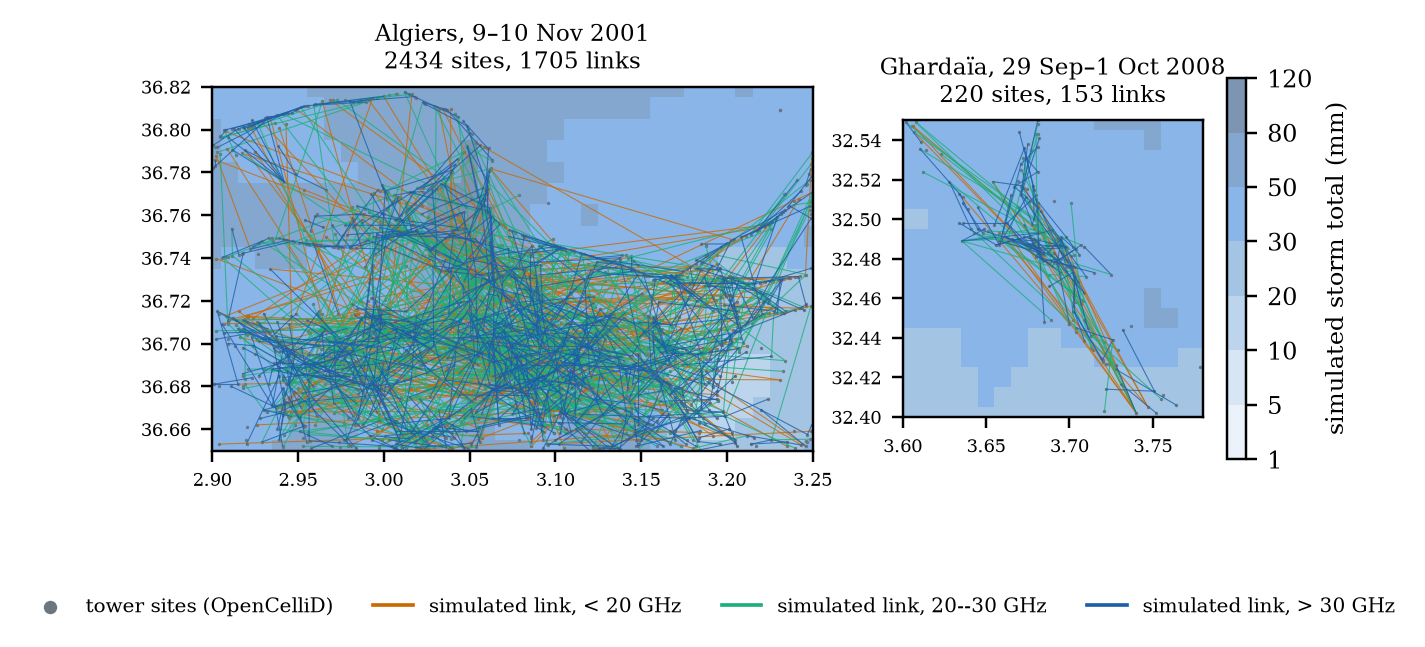
\includegraphics[width=\textwidth]{fig_p4_network.png}
\caption{Tower sites (grey dots) and the simulated links, coloured by frequency, over the simulated storm total. Algiers:
\PfourAlgSites{} sites, \PfourAlgLinks{} links, typical length \PfourAlgLenMed\,km (half between \PfourAlgLenLo{} and
\PfourAlgLenHi\,km). Ghardaïa: \PfourGhaSites{} sites, \PfourGhaLinks{} links, typical length \PfourGhaLenMed\,km. The empty
east of the Algiers box is the part of the tower download still to come.}
\label{fig:p4_network}
\end{figure}

\begin{careful}
\textbf{The network is probably too dense.} Real Algerian operators use fibre at more sites in the city centre, and split
sites inflate the count. So \PfourAlgLinks{} links in central Algiers is an upper bound. Section~\ref{sec:p4_density}
therefore repeats every map with only 50, 25, 10, 3 and 1\% of the links.
\end{careful}

%==========================================================
\section{Step 3: rain at the scale of a link}
\label{sec:p4_rain}
%==========================================================
A 5-km link inside one 10-km satellite square sees only part of it, and rain changes within minutes. So the satellite's
squares are turned into 1-km squares, every minute, in three moves:
\begin{enumerate}
\item \textbf{Motion.} From each pair of satellite images we measure how the rain moved (optical flow, as in
Section~\ref{sec:nowcast}). The typical speed was \PfourAlgSpeed\,km/h in Algiers and \PfourGhaSpeed\,km/h in Ghardaïa.
\item \textbf{Smooth in time.} Between two images, the rain is slid along that motion and blended, so it moves minute by
minute instead of jumping every 30 minutes.
\item \textbf{Detail inside each square.} The field is multiplied by a random pattern that is patchy at scales below
10\,km, drifts with the storm, and slowly changes. Its strength is \emph{measured}, not guessed: on the real 1-km radar of
Emilia-Romagna in November 2021 (an autumn Mediterranean month like the Algiers storm), we measured how much rain varies
inside a 10-km square, how much of it is wet, and how fast the pattern changes.
\end{enumerate}
Finally, each satellite square's amount over each half-hour is restored exactly: the simulation only \emph{adds detail},
it never changes the satellite's totals.

How the simulated rain compares with real radar rain (15-minute rain in 1-km squares, inside raining 10-km squares):
\begin{center}\footnotesize
\begin{tabular}{lccc}
\toprule
& real radar (Italy) & simulated, Algiers & simulated, Ghardaïa\\
\midrule
spread inside a 10-km square$^{*}$ & \PfourRadarSigma & \PfourAlgSigma & \PfourGhaSigma\\
share of the square that is wet & \PfourRadarWet & \PfourAlgWet & \PfourGhaWet\\
same pattern 15 minutes later$^{**}$ & \PfourRadarCorrA & \PfourAlgCorrA & \PfourGhaCorrA\\
same pattern 30 minutes later$^{**}$ & \PfourRadarCorrB & \PfourAlgCorrB & \PfourGhaCorrB\\
\bottomrule
\end{tabular}

\smallskip
{\footnotesize $^{*}$ standard deviation of the log of (1-km rain / 10-km average); 0.6 means a 1-km square is typically
within a factor of 1.8 of its 10-km average. $^{**}$ correlation of that pattern at the same place.}
\end{center}
The simulated rain is about as patchy as real rain and wet over a similar share, but clearly more persistent: its
pattern changes more slowly at a fixed place. Rain that changes slowly is easier to follow, so this flatters the system
(see the box at the end of this part). We set the pattern's strength once, on one test day, and did not tune it per storm.

%==========================================================
\section{Step 4: what each link would record}
\label{sec:p4_signal}
%==========================================================
For each sub-link and each minute, the recorded loss is built from four parts:
\begin{enumerate}
\item \textbf{Rain loss.} The rain is read every 100\,m along the beam and turned into loss with the ITU formula of
Section~\ref{sec:rain}, point by point, then added up. (Point by point matters: patchy rain along a beam does not cause the
same loss as the same amount spread evenly.)
\item \textbf{Wet antennas.} Water on the antenna covers adds loss: up to 1--2.5\,dB per link (drawn at random), building
up within minutes in rain and drying over about 45 minutes. The range matches the 1.5--2\,dB we found on Italian links in
long rain (Section~\ref{sec:may6}).
\item \textbf{A real recording underneath.} This is the key choice. Instead of inventing noise, each simulated sub-link
gets a real six-day recording from an Italian link during dry weather (radar rain less than 1\% of the time): its
noise, slow drifts, missing minutes, 1-dB steps, and its faults if it has any. The recordings come from the
\emph{eastern} half of the Italian network in 2022 (800 windows from 139 sub-links). The AI used here is the final recipe
trained on the \emph{western} half (Section~\ref{sec:newlinks}), so it has never seen this noise.
\item \textbf{Receiver floor and rounding.} A receiver cannot measure a signal weaker than about $-100$\,dBm (the Italian
recordings bottom out there), so in extreme rain the measured loss stops growing. Finally, the total is rounded to whole
decibels, like the recordings.
\end{enumerate}

\begin{figure}[h]
\centering
\begin{tikzpicture}
\begin{groupplot}[group style={group size=1 by 2,vertical sep=1.3cm,xlabels at=edge bottom},
  width=0.95\textwidth,height=4.2cm,xmin=0,xmax=48,grid=major,grid style={inkc!12},
  xtick={0,6,12,18,24,30,36,42,48},
  tick label style={font=\small},label style={font=\small},
  legend style={font=\scriptsize,draw=none,fill=white,fill opacity=0.85,text opacity=1},legend cell align=left]
\nextgroupplot[ylabel={rain (mm/h)},ymin=0,legend pos=north west]
  \addplot[thick,color=gaugec] table[x=hour,y=rtrue] {p4_link_algiers.dat};
  \addlegendentry{simulated truth along the link}
  \addplot[thick,color=rainc] table[x=hour,y=rai] {p4_link_algiers.dat};
  \addlegendentry{AI}
\nextgroupplot[ylabel={dB},xlabel={hours since 9 Nov 2001 00:00 UTC (30-minute averages)},ymin=-2,legend pos=north west]
  \addplot[thick,color=inkc] table[x=hour,y=excess] {p4_link_algiers.dat};
  \addlegendentry{recorded loss above the dry level}
  \addplot[thick,color=radarc,dashed] table[x=hour,y=rain_loss] {p4_link_algiers.dat};
  \addlegendentry{of which: rain}
  \addplot[thick,color=gaugec,densely dotted] table[x=hour,y=wet_antenna] {p4_link_algiers.dat};
  \addlegendentry{of which: wet antennas}
\end{groupplot}
\end{tikzpicture}
\caption{The wettest simulated sub-link in Algiers (\PfourAlgExLen\,km, \PfourAlgExFreq\,GHz) through the storm. Top: rain;
storm totals \PfourAlgExTrue\,mm (truth) and \PfourAlgExAI\,mm (AI). Bottom: what the link recorded, and the two parts that
the rain caused. The rest is the real recording underneath: noise, drift and 1-dB steps.}
\label{fig:p4_link}
\end{figure}

%==========================================================
\section{Step 5: the chain, and how it did}
\label{sec:p4_results}
%==========================================================
The simulated recordings go through exactly the steps of Parts~2 and~3, with no change for Algeria:
\begin{enumerate}
\item The \textbf{reliability score} (Section~\ref{sec:reliability}) keeps \PfourAlgReliable{} of \PfourAlgSub{} sub-links
in Algiers and \PfourGhaReliable{} of \PfourGhaSub{} in Ghardaïa. The rest are dropped, mostly because their real recordings
are faulty.
\item The \textbf{AI} (average of five runs) and the \textbf{classical method} turn each kept sub-link into rain.
\item \textbf{Hourly maps} by inverse-distance weighting (Section~\ref{sec:maps}), on the same 1-km squares as the truth.
\end{enumerate}
Scores cover the storm days only (the three dry days before are needed for the dry level, not judged).

\begin{figure}[h]
\centering
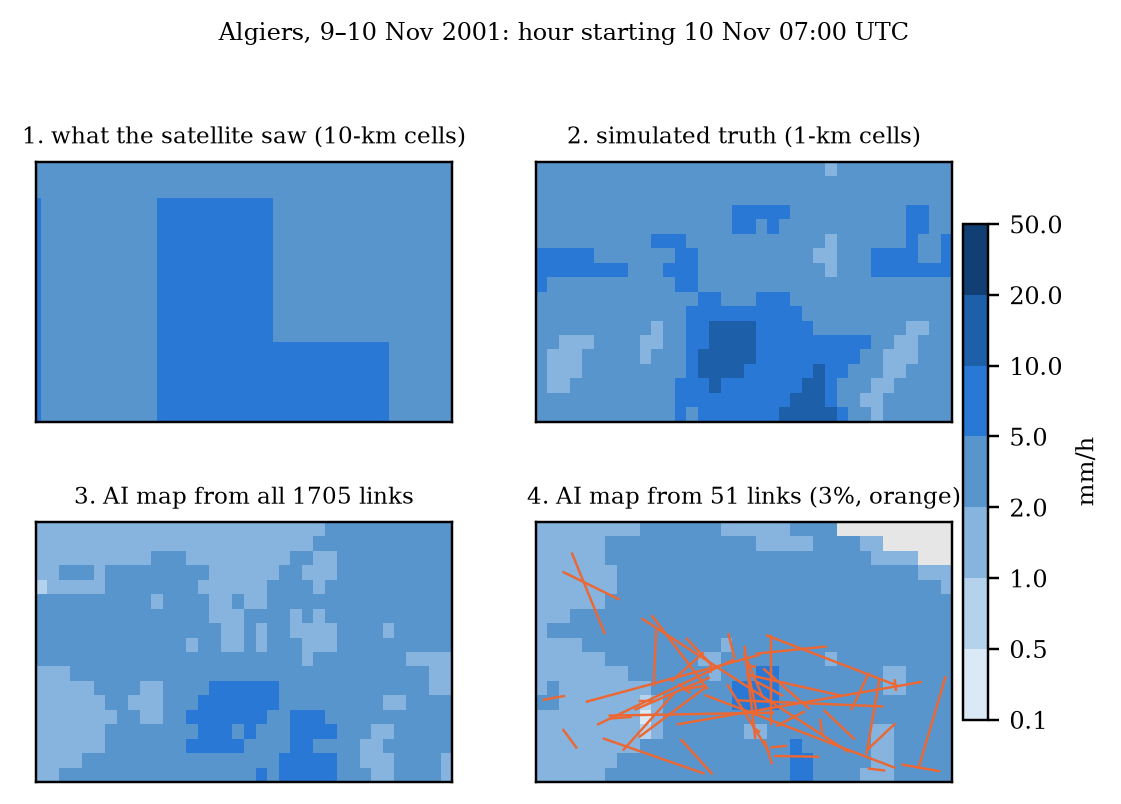
\includegraphics[width=0.92\textwidth]{fig_p4_steps_algiers.png}
\caption{The wettest hour in Algiers (\PfourAlgHour{} UTC), from satellite to map. 1: the satellite's 10-km squares. 2: the
simulated truth after Step~3. 3: the AI map from all links. 4: the AI map from only 3\% of the links (orange).}
\label{fig:p4_steps}
\end{figure}

\begin{figure}[h]
\centering
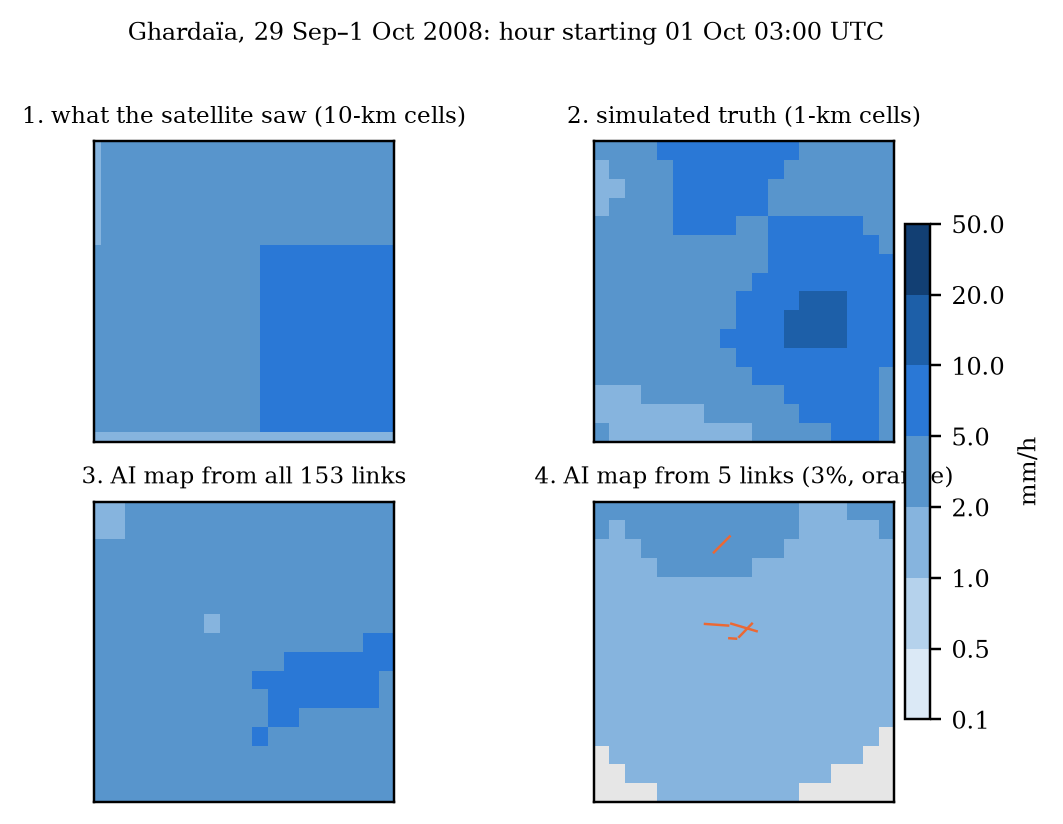
\includegraphics[width=0.75\textwidth]{fig_p4_steps_ghardaia.png}
\caption{The same four steps for the wettest hour in Ghardaïa (\PfourGhaHour{} UTC). The town is small, so a 10-km
satellite square covers most of it; the links add the detail inside.}
\label{fig:p4_steps_gha}
\end{figure}

\begin{center}\footnotesize\setlength{\tabcolsep}{4pt}
\begin{tabular}{llcccc}
\toprule
& & \multicolumn{2}{c}{\textbf{per link}} & \multicolumn{2}{c}{\textbf{map (1-km squares)}}\\
\cmidrule(lr){3-4}\cmidrule(lr){5-6}
City & method & hourly correlation & storm total & hourly correlation & storm total\\
\midrule
Algiers & AI & \PfourAlgAILinkR & \PfourAlgAILinkBias & \PfourAlgAIMapR & \PfourAlgAIMapBias\\
& classical & \PfourAlgClLinkR & \PfourAlgClLinkBias & \PfourAlgClMapR & \PfourAlgClMapBias\\
Ghardaïa & AI & \PfourGhaAILinkR & \PfourGhaAILinkBias & \PfourGhaAIMapR & \PfourGhaAIMapBias\\
& classical & \PfourGhaClLinkR & \PfourGhaClLinkBias & \PfourGhaClMapR & \PfourGhaClMapBias\\
\bottomrule
\end{tabular}
\end{center}

\begin{itemize}
\item \textbf{The AI tracks rain much better link by link} (hourly correlation \PfourAlgAILinkR{} against
\PfourAlgClLinkR{} in Algiers). The real recordings underneath are full of drifts and steps that the classical method
mistakes for rain; the AI, trained on such recordings, does not.
\item \textbf{On the map the two methods look alike}, because averaging many links smooths out each link's errors.
\item \textbf{The AI measures too little, as it did in Sweden and Italy.} In Algiers it finds \PfourAlgAICityTot{} of the
city's \PfourAlgTruthTot\,mm. The shortfall sits in the heavier and longer rain: hours of 2\,mm/h or more, and the second
day of the storm. These are the two weaknesses found in Part~2 (Sections~\ref{sec:se_results} and~\ref{sec:may6}); the
simulation shows them again, it did not create them.
\end{itemize}

\subsection{How many links are enough?}
\label{sec:p4_density}
Because the simulated network is probably denser than the real one, we repeated the AI maps with a random share of the
links:
\begin{center}
\begin{tikzpicture}
\begin{axis}[width=0.7\textwidth,height=5cm,xmode=log,xmin=0.008,xmax=1.2,ymin=0.5,ymax=1,
  xtick={0.01,0.03,0.1,0.25,0.5,1},xticklabels={1\%,3\%,10\%,25\%,50\%,100\%},
  xlabel={share of the simulated links used},ylabel={hourly correlation, map vs truth},
  grid=major,grid style={inkc!12},tick label style={font=\small},label style={font=\small},
  legend style={font=\scriptsize,draw=none,at={(0.98,0.04)},anchor=south east},legend cell align=left]
\addplot[thick,color=rainc,mark=*,mark size=1.5pt] table[x=frac,y=algiers_ai_r] {p4_density.dat};
\addlegendentry{Algiers, AI}
\addplot[thick,color=gaugec,mark=square*,mark size=1.5pt] table[x=frac,y=ghardaia_ai_r] {p4_density.dat};
\addlegendentry{Ghardaïa, AI}
\end{axis}
\end{tikzpicture}
\end{center}
Even 3\% of the Algiers links (\PfourAlgSparseN{} links) give a map with hourly correlation \PfourAlgAISparseR{}, covering
\PfourAlgAISparseCover{} of the city. With so few links, where a square is matters: within 1\,km of a link the correlation is
\PfourAlgDistA, at 2--5\,km \PfourAlgDistC, at 5--10\,km \PfourAlgDistD.

\begin{careful}
\textbf{Why these numbers flatter the system.}
\begin{itemize}
\item \textbf{The storms are smoothed.} The truth is built from 10-km satellite rain plus measured patchiness, so it has no
small, violent cells hidden between links. Real flash floods often come from exactly such cells.
\item \textbf{The rain changes too slowly.} The simulated pattern stays in place longer than real rain does (Step~3
table), which makes each link's view more representative of the area around it.
\item \textbf{The physics matches.} The rain loss is computed with the same ITU formula the methods use to turn loss back
into rain. Real drop sizes vary, and with them the true formula.
\item \textbf{Mild storms.} Satellite averages rarely push links to their limit, so outages in extreme rain barely appear.
\end{itemize}
In the other direction, two things are \emph{harder} than reality: the AI has never seen these links' noise, and no
Algerian data was used to tune anything.
\end{careful}

\begin{oneline}
On real Algerian tower positions, with real storms and real link noise, the whole chain runs and gives city rain maps
that follow the simulated truth closely (hourly correlation \PfourAlgAIMapR{} in Algiers), even with a few dozen links; the AI
still measures \PfourAlgAIMapBias{} too little in a two-day storm. Real accuracy in Algeria remains to be shown with an
operator's data.
\end{oneline}

%==========================================================
\section{Every choice, and why}
\label{sec:p4_choices}
%==========================================================
\begin{center}\footnotesize\setlength{\tabcolsep}{4pt}
\begin{tabular}{>{\raggedright\arraybackslash}p{2.8cm}>{\raggedright\arraybackslash}p{3.6cm}>{\raggedright\arraybackslash}p{6.9cm}}
\toprule
Choice & Value & Why, and how it was checked\\
\midrule
Storms & Algiers Nov 2001, Ghardaïa Oct 2008 & one coastal city, one desert wadi; both floods are well documented (Section~\ref{sec:p4_storms}
on the satellite's timing)\\
Rain source & NASA IMERG V07, 30 min, 10 km & the only rain data covering Algeria since 1998, free\\
Spin-up & 3 dry days before each storm & the AI's dry level looks back 3 days\\
Tower positions & OpenCelliD, sites = antennas within 150\,m & only public source; approximate (Section~\ref{sec:p4_network})\\
Hubs (fibre) & 30\% of sites & unknown in Algeria; the density test covers 1--100\% of links\\
Hop lengths & drawn from Gothenburg + Netherlands & real city networks; nearest-neighbour links would be 0.5\,km, far too short\\
Frequency, polarisation & copied from a real link of similar length & keeps the real link between length and frequency\\
Rain grid & 1\,km, 1 minute & the scale of a link and of its readings\\
Patchiness & strength 0.6, renewal 20 min & set so 15-min, 1-km statistics match real radar (Step~3 table)\\
Satellite amounts & restored per square and half-hour & the simulation adds detail only\\
Rain loss & ITU-R P.838, every 100\,m along the beam & standard formula; point by point for patchy rain\\
Wet antennas & 1--2.5\,dB, dries in 45 min & matches Italian links in long rain\\
Noise & real dry recordings, eastern Italy 2022 & real noise is harder than invented noise; the AI never saw these links\\
Receiver floor & $-100$\,dBm & where the Italian recordings bottom out\\
AI & final recipe, western Italy, 5 runs & clean separation from the noise source\\
Maps & IDW, 8 links within 10\,km & unchanged from Part~3\\
\bottomrule
\end{tabular}
\end{center}

\textbf{Next:} Phase~5 turns these rain maps into flood risk: where the water goes (terrain, wadis), how much ground is
sealed by concrete, and who lives there.
